\documentclass[12pt,reqno]{amsart}
\usepackage[top=2cm, left=2cm,right=2cm,bottom=2cm]{geometry}
\renewcommand{\baselinestretch}{1.2}
\usepackage{amsmath}
\usepackage{amssymb}
\usepackage{scalefnt}
\usepackage{tikz}
\usepackage{color,hyperref,enumerate,multicol}
\definecolor{darkblue}{rgb}{0.0,0.0,0.3}
\hypersetup{colorlinks,breaklinks,
            linkcolor=darkblue,urlcolor=darkblue,
            anchorcolor=darkblue,citecolor=darkblue}
            
\usepackage{algorithm}
\usepackage{algorithmic}
\pagestyle{empty}
\newcommand{\N}{\ensuremath{\mathbb{N}}}
\newcommand{\Z}{\ensuremath{\mathbb{Z}}}
\newcommand{\R}{\ensuremath{\mathbb{R}}}
\newcommand{\bL}{\ensuremath{\mathbf{L}}}
\newcommand{\bP}{\ensuremath{\mathbf{P}}}
\newcommand{\bQ}{\ensuremath{\mathbf{Q}}}
\newcommand{\bA}{\ensuremath{\mathbf{A}}}
\newcommand{\bB}{\ensuremath{\mathbf{B}}}
\newcommand{\bG}{\ensuremath{\mathbf{G}}}
\newcommand{\bH}{\ensuremath{\mathbf{H}}}
\newcommand{\invG}{\ensuremath{\operatorname{inv}^{\bG}}}
\newcommand{\invH}{\ensuremath{\operatorname{inv}^{\bH}}}
\newcommand{\meet}{\ensuremath{\wedge}}
\newcommand{\Meet}{\ensuremath{\bigwedge}}
\newcommand{\<}{\ensuremath{\langle}}
\renewcommand{\>}{\ensuremath{\rangle}}
\newcommand{\join}{\ensuremath{\vee}}
\renewcommand{\emptyset}{\ensuremath{\varnothing}}
\renewcommand{\subset}{\ensuremath{\subsetneq}}
\newcommand{\boldemph}{\emph}
\newcommand{\lcm}{\operatorname{lcm}}

\newcommand{\probskip}{\vskip1cm}

\begin{document}
\thispagestyle{empty}

\noindent \textbf{Math 301} \hskip5cm {\bf Homework 9} \hfill {\bf Fall 2014}
\vskip1cm
\noindent {\bf Exercises:} 1, 2, 3 below and Judson: 9.22, 9.27, 9.31\\
{\bf Recommended:} 9.19, 9.21, 9.23, 9.41, 9.42, 9.45\\
{\bf Due date:} Friday, 10/31

\bigskip

\noindent The first few exercises require some definitions from lecture, 
repeated here for your convenience.

\vskip5mm

\noindent Let $\bA = \<A, F^{\bA}\>$ and $\bB = \<B, F^{\bB}\>$ be two algebras of the
same \emph{similarity type}.  That is, to each operation
symbol $f \in F$ there corresponds an operation $f^{\bA}$ defined on $\bA$ and an
operation $f^{\bB}$ defined on $\bB$.
Thus, the set of operations defined on $\bA$ is the set 
$F^{\bA} = \{f^{\bA} : f\in F\}$; similarly 
$F^{\bB} = \{f^{\bB} : f\in F\}$.

\vskip3mm

\noindent For example, any two groups $\bG$ and $\bH$ have the same similarity type. 
To emphasize this, we could denote the operations of these groups using
the precise (albeit somewhat awkward) notation of the previous paragraph, as follows:
\[
\bG  = \<G, \circ^{\bG}, \invG, e^{\bG}\> \quad \text{ and } \quad
\bH  = \<H, \circ^{\bH}, \invH, e^{\bH}\>.
\] 
Here $\circ^{\bG}$, $\invG$, and $e^{\bG}$ represent the \emph{interpretation
in} $\bG$ of the binary, unary (inverse), and  nullary (identity)
operations that a group must possess (similarly for $\bH$).  

\vskip5mm

\noindent An \emph{algebra homomorphism} (or simply \emph{homomorphism}), denoted by
$\varphi: \bA \rightarrow \bB$, is a function $\varphi$ with domain $A$ and
codomain $B$ that satisfies the following conditions: for each $f \in F$, if $f$
is an $n$-ary operation symbol, and if $a_1, \dots, a_n \in A$, then
\[
\varphi(f^{\bA}(a_1, \dots, a_n)) = f^{\bB}(\varphi(a_1), \dots, \varphi(a_n)).
\]

\vskip3mm

\noindent For example, a \emph{group homomorphism} $\varphi: \bG \rightarrow \bH$  is a function 
$\varphi$ with domain $G$ and codomain $H$ that satisfies, $\forall x, y \in G$,
\begin{enumerate}
\item  $\varphi(x\circ^{\bG} y) = \varphi(x) \circ^{\bH} \varphi(y)$,
\item  $\varphi(\invG(x)) = \invH(\varphi(x))$,
\item  $\varphi(e^{\bG}) = e^{\bH}$.
\end{enumerate}

\vskip5mm

\noindent The textbook defines a group \emph{isomorphism} to be a group homomorphism that is both
one-to-one and onto.  This definition is fine for algebraic structures (like
groups).  
It does not work, however, for relational structures, like posets. (See Exercise 3 below).
A definition that works for both algebraic and relational structures is the following:
A homomorphism $\varphi : \bA \rightarrow \bB$ is an \emph{isomorphism} if there
exists a homomorphism $\psi: \bB \rightarrow \bA$ that composes with
$\varphi$ to give the identity, that is,
$\varphi \circ \psi = \operatorname{id}_B$
and $\psi \circ \varphi= \operatorname{id}_A$. (Here, $\operatorname{id}_X$
denotes the identity function on the set $X$: $\operatorname{id}_X(x) = x$.)

\newpage

\noindent {\bf Exercises}

\begin{enumerate}[{\bf 1.}]
%% 1 %%%%%%%%%%%%%%%%%%%%%%%%%%%%%%%%%%%%%%%%%%%%%%%%
\item When discussing two groups, like $\bG$ and $\bH$ above,
  our textbook uses more convenient notation, such as 
  $(G, \cdot)$ and $(H, \circ)$ (or, even more simply, $G$ and $H$).  The book will then
  define a \emph{homomorphism} to be a function $\varphi: G\rightarrow H$ satisfying
  $\varphi(x\cdot y) = \varphi(x) \circ \varphi(y)$.
  Prove that this is equivalent to the definition given above by showing that 
  conditions (2) and (3) are unnecessary.\\
  \ [Hint: Assuming (1), derive (3), then derive (2).]

\vskip1cm

%% 2 %%%%%%%%%%%%%%%%%%%%%%%%%%%%%%%%%%%%%%%%%%%%%%%%
\item
Define a lattice homomorphism.
Then consider a lattice $\bL = \<L, \meet, \join\>$ and a poset $\bP = \<P, \preccurlyeq\>$.
Is it possible to define a homomorphism $\varphi: \bL \rightarrow \bP$?  Explain.

\vskip1cm

%% 3 %%%%%%%%%%%%%%%%%%%%%%%%%%%%%%%%%%%%%%%%%%%%%%%%
\item
A \emph{poset homomorphism} is an order preserving map.  That is, if
$\bP = \<P, \leqslant\>$ and 
$\bQ = \<Q, \preccurlyeq\>$ are two partially 
ordered sets, then a homomorphism 
$\varphi: \bP \rightarrow \bQ$  is a function satisfying, for all $x, y\in P$, 
if $x \leqslant y$ then $\varphi(x)\preccurlyeq \varphi(y)$.
Consider the two definitions of \emph{isomorphism} given in the last paragraph
on Page 1 above.
Using the two posets shown below, explain why the first of these definitions is 
not appropriate for posets.

\vskip5mm

\begin{center}
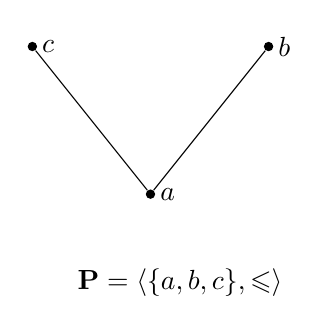
\begin{tikzpicture}[scale=0.75]
  \node (0) at (0,.5) [fill,circle,inner sep=1.2pt] {};
  \node (1) at (2,3) [fill,circle,inner sep=1.2pt] {};
  \node (2) at (-2,3) [fill,circle,inner sep=1.2pt] {};
  \draw (0) node [right] {$a$};
  \draw (1) node [right] {$b$};
  \draw (2) node [right] {$c$};
  \node (3) at (0.5,-1) {$\bP = \<\{a,b,c\},  \leqslant\>$};
  \draw (1) to (0) to (2);
\end{tikzpicture}
\hskip3cm
\begin{tikzpicture}[scale=0.75]
  \node (0) at (0,0) [fill,circle,inner sep=1.2pt] {};
  \node (1) at (0,2) [fill,circle,inner sep=1.2pt] {};
  \node (2) at (0,4) [fill,circle,inner sep=1.2pt] {};
  \draw (0) node [right] {$0$};
  \draw (1) node [right] {$1$};
  \draw (2) node [right] {$2$};
  \node (3) at (0.5,-1.5) {$\bQ = \<\{0,1,2\}, \preccurlyeq\>$};
  \draw (0) to (1) to (2);
\end{tikzpicture}
\end{center}

\vskip1cm

%% %% 7 %%%%%%%%%%%%%%%%%%%%%%%%%%%%%%%%%%%%%%%%%%%%%%%%
%% \item[{\bf 9.7.}] 
%% Show that any cyclic group of order $n$ is isomorphic to ${\mathbb Z}_n$. 

\vskip1cm

\item[{\bf 9.22}]
Let $G$ be a group of order 20. If $G$ has subgroups $H$ and $K$ of
orders 4 and 5 respectively such that $hk = kh$ for all $h \in H$ and
$k \in K$, prove that $G$ is the internal direct product of $H$ and $K$. 

\vskip1cm

\item[{\bf 9.27}]
Let $G \cong H$. Show that if $G$ is cyclic, then so is $H$.

\vskip1cm

\item[{\bf 9.31}]
Let $\phi : G_1 \rightarrow G_2$ and  $\psi : G_2 \rightarrow G_3$  be
isomorphisms. Show that  $\phi^{-1}$ and $\psi \circ \phi$ are both
isomorphisms. Using these results, show that the isomorphism of groups
determines an equivalence relation on the class of all groups.
 
\end{enumerate}
\end{document}
